\documentclass[a4paper]{article}
% generated by Docutils <http://docutils.sourceforge.net/>
\usepackage{fixltx2e} % LaTeX patches, \textsubscript
\usepackage{cmap} % fix search and cut-and-paste in Acrobat
\usepackage{ifthen}
\usepackage[T1]{fontenc}
\usepackage[utf8]{inputenc}
\usepackage{float} % float configuration
\floatplacement{figure}{H} % place figures here definitely
\usepackage{graphicx}
\usepackage{longtable,ltcaption,array}
\setlength{\extrarowheight}{2pt}
\newlength{\DUtablewidth} % internal use in tables
\usepackage{tabularx}

%%% Custom LaTeX preamble
% PDF Standard Fonts
\usepackage{mathptmx} % Times
\usepackage[scaled=.90]{helvet}
\usepackage{courier}

%%% User specified packages and stylesheets

%%% Fallback definitions for Docutils-specific commands

% providelength (provide a length variable and set default, if it is new)
\providecommand*{\DUprovidelength}[2]{
  \ifthenelse{\isundefined{#1}}{\newlength{#1}\setlength{#1}{#2}}{}
}

% docinfo (width of docinfo table)
\DUprovidelength{\DUdocinfowidth}{0.9\textwidth}

% hyperlinks:
\ifthenelse{\isundefined{\hypersetup}}{
  \usepackage[colorlinks=true,linkcolor=blue,urlcolor=blue]{hyperref}
  \urlstyle{same} % normal text font (alternatives: tt, rm, sf)
}{}
\hypersetup{
  pdftitle={Pweave Example - Frequency response of a moving average filter},
  pdfauthor={Matti Pastell <matti.pastell@helsinki.fi>}
}

%%% Title Data
\title{\phantomsection%
  Pweave Example - Frequency response of a moving average filter%
  \label{pweave-example-frequency-response-of-a-moving-average-filter}}
\author{}
\date{}

%%% Body
\begin{document}
\maketitle

% Docinfo
\begin{center}
\begin{tabularx}{\DUdocinfowidth}{lX}
\textbf{Author}: &
	Matti Pastell <\href{mailto:matti.pastell@helsinki.fi}{matti.pastell@helsinki.fi}> \\
\textbf{Website}: &
\url{http://mpastell.com}
\\
\end{tabularx}
\end{center}

\textbf{Create 11 point moving average filter and plot its frequency response and print the values.}
%
\begin{quote}{\ttfamily \raggedright \noindent
from~pylab~import~*\\
import~scipy.signal~as~signal\\
\#A~function~to~plot~frequency~and~phase~response\\
def~mfreqz(b,a=1):\\
~~~~w,h~=~signal.freqz(b,a)\\
~~~~h~=~abs(h)\\
~~~~return(w/max(w),~h)
}
\end{quote}

\textbf{Make the impulse response function and use terminal formatted output (=doctest block.)}
%
\begin{quote}{\ttfamily \raggedright \noindent
>{}>{}>~n~=~11.\\
>{}>{}>~n\\
11.0\\
>{}>{}>~b~=~repeat(1/n,~n)\\
>{}>{}>~b\\
array({[}~0.09090909,~~0.09090909,~~0.09090909,~~0.09090909,~~0.09090909,\\
~~~~~~~~0.09090909,~~0.09090909,~~0.09090909,~~0.09090909,~~0.09090909,\\
~~~~~~~~0.09090909{]})
}
\end{quote}

\textbf{Calculate the frequency response and plot it:}
%
\begin{quote}{\ttfamily \raggedright \noindent
w,~h~=~mfreqz(b)\\
\#Plot~the~function\\
plot(w,h,'k')\\
ylabel('Amplitude')\\
xlabel(r'Normalized~Frequency~(x\$\textbackslash{}pi\$rad/sample)')\\
show()
}
\end{quote}
\begin{figure}
\noindent\makebox[\textwidth][c]{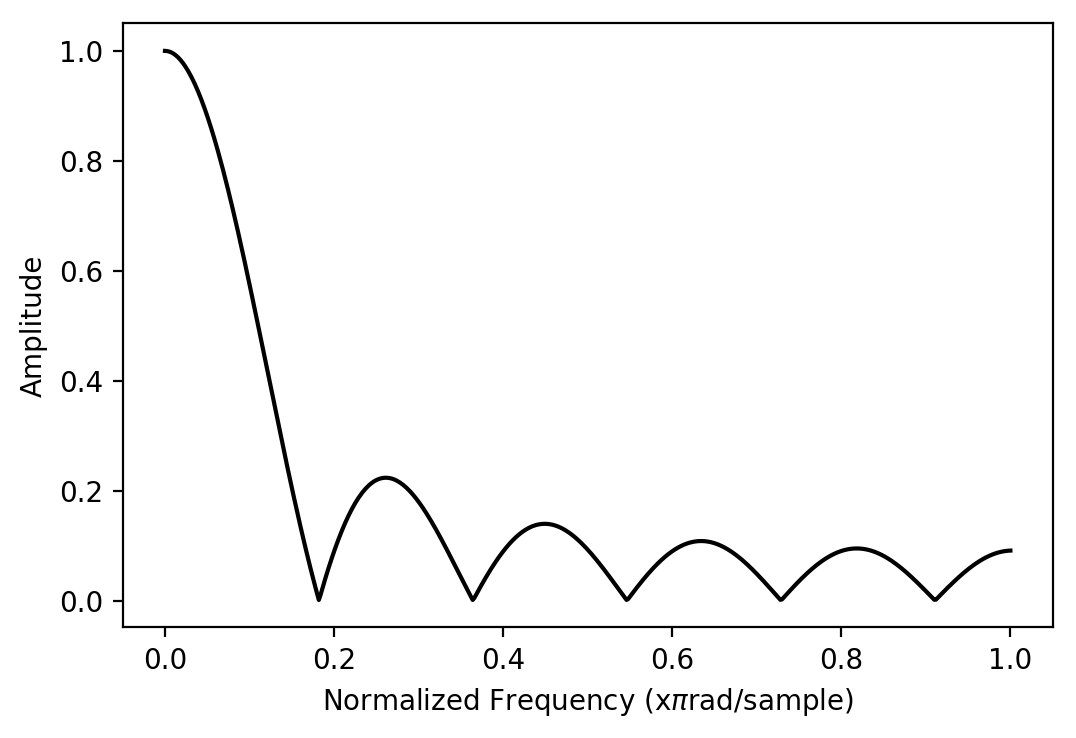
\includegraphics[width=15cm]{figures/ma_figure3_1.png}}
\caption{Frequency response of an 11 point moving average filter}
\end{figure}

\textbf{The first 10 values of the frequency response (w,h) as a table, notice that the code is hidden in the output document.}

\setlength{\DUtablewidth}{\linewidth}
\begin{longtable*}[c]{|p{0.191\DUtablewidth}|p{0.191\DUtablewidth}|}
\hline
\textbf{%
Amplitude
} & \textbf{%
Frequency
} \\
\hline
\endfirsthead
\hline
\textbf{%
Amplitude
} & \textbf{%
Frequency
} \\
\hline
\endhead
\multicolumn{2}{c}{\hfill ... continued on next page} \\
\endfoot
\endlastfoot

1.0
 & 
0.0
 \\
\hline

1.0
 & 
0.0
 \\
\hline

1.0
 & 
0.0
 \\
\hline

1.0
 & 
0.01
 \\
\hline

1.0
 & 
0.01
 \\
\hline

1.0
 & 
0.01
 \\
\hline

0.99
 & 
0.01
 \\
\hline

0.99
 & 
0.01
 \\
\hline

0.99
 & 
0.02
 \\
\hline

0.98
 & 
0.02
 \\
\hline
\end{longtable*}

\end{document}
